\section{Appendix B: Artifacts}
Our code is version-controlled on GitHub. We provide a README and commented code 
at \url{https://github.com/code-correctional-facility/deepbugs-jr}.

\iffalse
\label{sec:appendix_b}
The purpose of our project is to reproduce the DeepBugs study to substantiate the authors' claim  of name-based bug detection through machine learning. To do so, we will follow the study's approach to using a TensorFlow machine learning model. Our team has set up a repository on Github where our project will be hosted and tracking tasking through a kanban board on Jira. The team will proceed to assess the requirements specified in the study. Once completed, we will begin compiling tasks for the project backlog. At this stage, development of the neural network layers will commence. 

As explained in Section \ref{sec:timeline}, our team will use Scrum for day-to-day operations. However, we do plan to create most of the requirements at the start of the project and follow the macro flow process shown in Figure \ref{fig:engineering_process}.

\begin{figure}[ht]
    \centering
    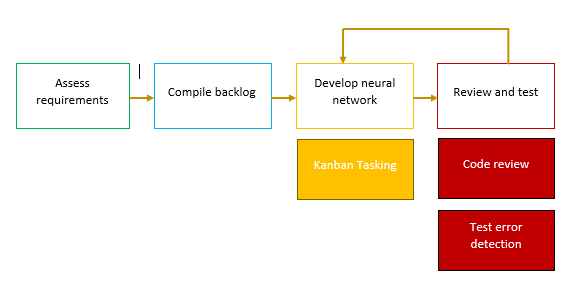
\includegraphics[width=\linewidth]{images/Engineering Process.PNG}
    \caption{Project Flow Overview}
    \label{fig:engineering_process}
\end{figure}

Our team has established a scheduled meeting on a weekly basis which will be used to assign tasks and provide status updates for work in progress. In the spirit of following suit with \textit{Software Engineering at Google}'s approach to code review, we will require changes to source code receive a "looks good to me" from any other member of the team.

Lastly, relevant works used in the development of our reproduction will be tracked in Zotero. This tool will allow the team to maintain a list of works which will be cited as resources.

\fi